\section{Initial Software Setup}
This section details the configuration of the key software and packages within the pipeline. The installation 
processes of Miniconda and Docker are very lengthy and can therefore be found in Appendix A.

\subsection{VirtualBox \& Ubuntu}
The majority of data scientists utilise Linux distributions for their projects due to its open-source nature and the 
availability of many tools and packages. Therefore, VirtualBox, software to create a virtual machine which runs inside the host 
machine \autocite{oracle_oracle_nodate}, will be used to virtualise an Ubuntu 22.04 LTS system on the Windows host machine. This 
particular OS was chosen because of its relative recency and frequent software \& security updates. Virtual machines
also allow for "snapshots", which store the current state of the machine and its files at that time to be restored at any point in the 
event of unforeseen errors. Should a catastrophic error that would damage the system occur, the host machine would be unaffected as the 
virtual machine is isolated.

\begin{figure}[H]
    \centering
    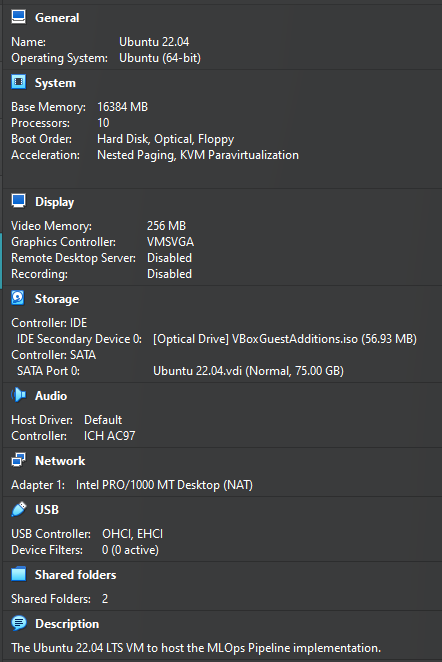
\includegraphics[width=.5\linewidth]{Implementation/VBoxConfig.png}
    \caption{The configuration for the pipeline's VM.}
    \label{fig:VBoxConfig}
\end{figure}

\begin{figure}[H]
    \centering
    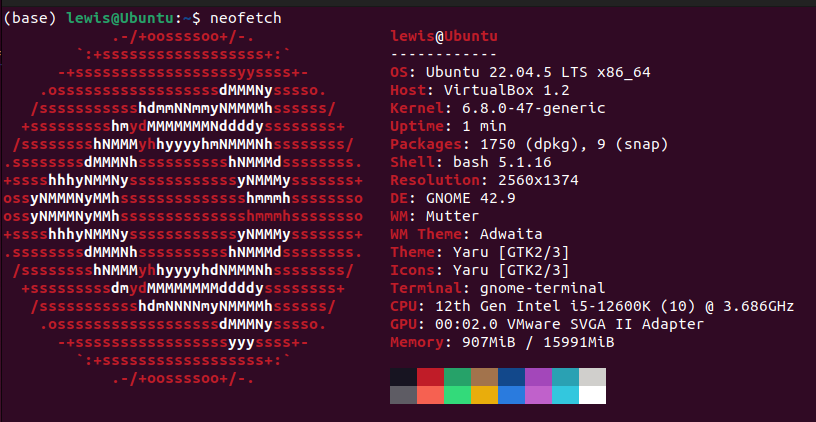
\includegraphics[width=.75\linewidth]{Implementation/Neofetch.png}
    \caption{The VM's Neofetch display.}
    \label{fig:Neofetch}
\end{figure}

\subsection{Conda environment and packages}
This section details the installation of packages to the Pipeline environment.

\begin{figure}[H]
    \centering
    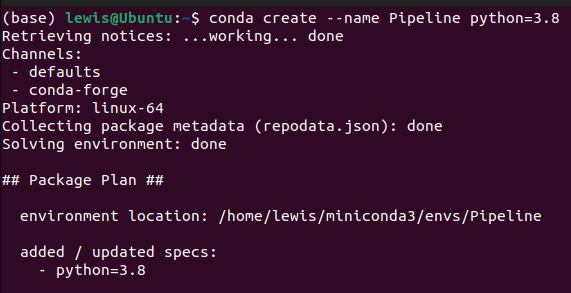
\includegraphics[width=.75\linewidth]{Implementation/Conda/CondaCreation.png}
    \caption{Creating the "Pipeline" Conda environment.}
    \label{fig:CondaCreation}
\end{figure}

\para Python 3.9.7 is used due to package compatibility issues with later versions of Python.

\begin{figure}[H]
    \centering
    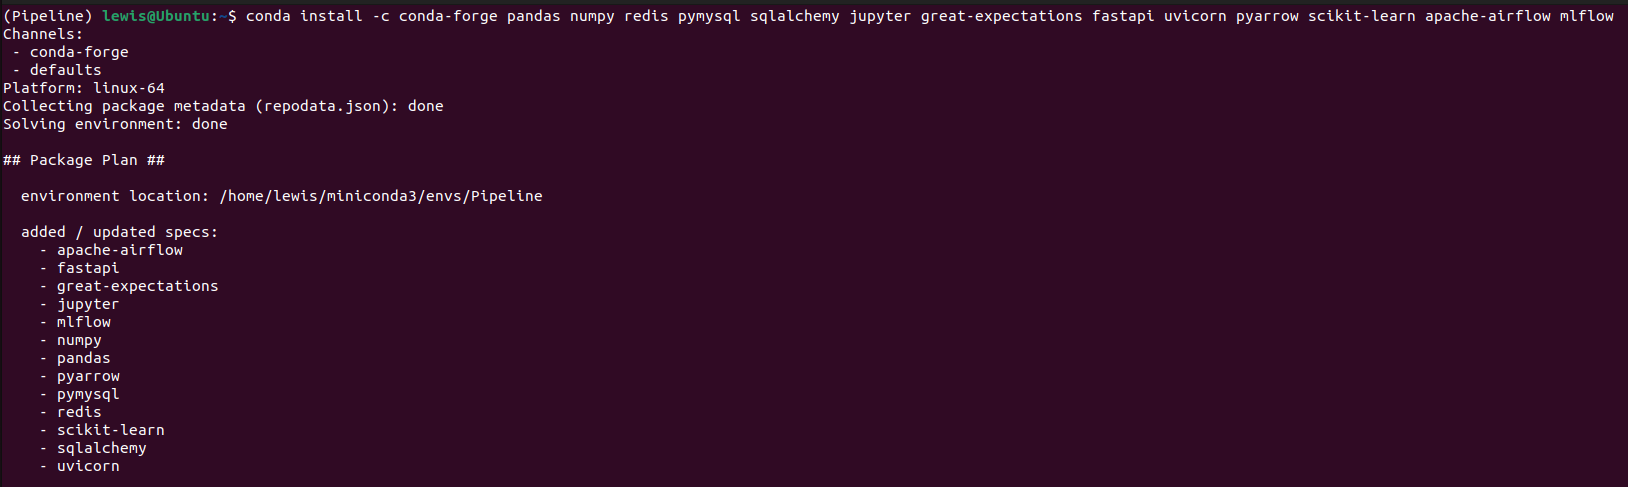
\includegraphics[width=\linewidth]{Implementation/Conda/CondaPackages.png}
    \caption{Installing packages to the environment via Conda.}
    \label{fig:CondaPackages}
\end{figure}

\subsection{Docker and Docker images}
This section covers the downloading of the two necessary Docker images, MariaDB Columnstore and Redis. 
Their usage is further elaborated upon later in this chapter. The images for the containers will first need to be
downloaded from Docker's repository, shown in Figure \ref{fig:DockerPull}.

\begin{figure}[H]
    \centering
    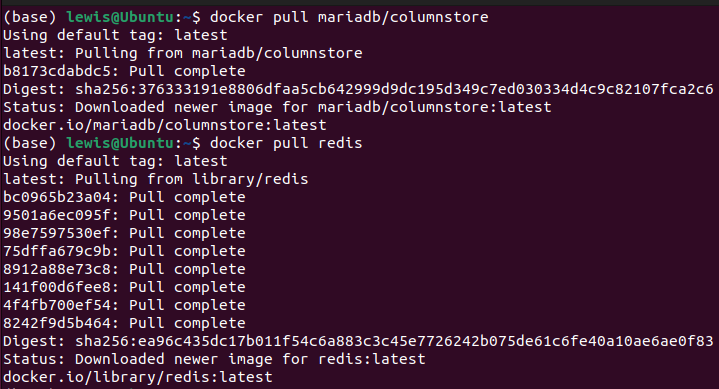
\includegraphics[width=\linewidth]{Implementation/Docker/Containers/Pull.png}
    \caption{Pulling the Docker images.}
    \label{fig:DockerPull}
\end{figure}

\pagebreak 
\subsubsection{MariaDB Columnstore}
MariaDB Columnstore runs on port 3306, but is mapped to port 3307 to avoid a possible Docker error.

\begin{figure}[H]
    \centering
    \includegraphics[width=\linewidth]{Implementation/Docker/Containers/MariaDB/1.png}
    \caption{Creating the MariaDB Columnstore container.}
    \label{fig:CreateMCS}
\end{figure}

\begin{figure}[H]
    \centering
    \includegraphics[width=\linewidth]{Implementation/Docker/Containers/MariaDB/2.png}
    \caption{Creating the user account for MariaDB.}
    \label{fig:CreateMCSUser}
\end{figure}

\begin{figure}[H]
    \centering
    \includegraphics[width=\linewidth]{Implementation/Docker/Containers/MariaDB/3.png}
    \caption{Creating the database for later use.}
    \label{fig:CreateDB}
\end{figure}

\pagebreak 
\subsubsection{Redis}
Redis runs on port 6379.

\begin{figure}[H]
    \centering
    \includegraphics[width=\linewidth]{Implementation/Docker/Containers/Redis/1.png}
    \caption{Creating the Redis container.}
    \label{fig:CreateRedis}
\end{figure}


\subsection{Airflow and MLFlow initialisation}
Airflow and MLFlow do not immediately work upon install, and must first be initialised.

\subsubsection{Airflow}
\begin{figure}[H]
    \centering
    \includegraphics[width=\linewidth]{Implementation/Airflow/Initialisation/1.png}
    \caption{Initialising Airflow's database.}
    \label{fig:AirflowInit}
\end{figure}

\begin{figure}[H]
    \centering
    \includegraphics[width=\linewidth]{Implementation/Airflow/Initialisation/2.png}
    \caption{Creating an administrative Airflow user.}
    \label{fig:AirflowUser1}
\end{figure}

\begin{figure}[H]
    \centering
    \includegraphics[width=\linewidth]{Implementation/Airflow/Initialisation/3.png}
    \caption{Verifying that the user was created.}
    \label{fig:AirflowUser2}
\end{figure}

\begin{figure}[H]
    \centering
    \includegraphics[width=\linewidth]{Implementation/Airflow/Initialisation/4.png}
    \caption{Successfully starting Airflow's web server.}
    \label{fig:AirflowWebserver}
\end{figure}

\begin{figure}[H]
    \centering
    \includegraphics[width=\linewidth]{Implementation/Airflow/Initialisation/5.png}
    \caption{Successfully starting Airflow's task scheduler.}
    \label{fig:AirflowScheduler}
\end{figure}

\subsubsection{MLFlow}

\begin{figure}[H]
    \centering
    \includegraphics[width=\linewidth]{Implementation/MLFlow/Initialisation/1.png}
    \caption{Creating a directory for MLFlow and initialising its database.}
    \label{fig:MLFlowInit}
\end{figure}

\begin{figure}[H]
    \centering
    \includegraphics[width=\linewidth]{Implementation/MLFlow/Initialisation/3.png}
    \caption{Running MLFlow's frontend web UI.}
    \label{fig:MLFlowUICmd}
\end{figure}

\begin{figure}[H]
    \centering
    \includegraphics[width=\linewidth]{Implementation/MLFlow/Initialisation/2.png}
    \caption{MLFlow's web UI.}
    \label{fig:MLFlowEmptyUI}
\end{figure}

\subsection{Great Expectations}

\begin{figure}[H]
    \centering
    \includegraphics[width=\linewidth]{Implementation/GX/Initialisation/1.png}
    \caption{Checking the installed GX version and initialising it.}
    \label{fig:GXVersion}
\end{figure}

\begin{figure}[H]
    \centering
    \includegraphics[width=\linewidth]{Implementation/GX/Initialisation/2.png}
    \caption{Confirmation of the successful initialisation.}
    \label{fig:GXInitConfirm}
\end{figure}

% \begin{figure}[H]
%     \centering
%     \includegraphics[width=\linewidth]{Implementation/GX/Initialisation/3.png}
%     \caption{Viewing the contents of the created directory.}
%     \label{fig:GXDir}
% \end{figure}

\begin{figure}[H]
    \centering
    \includegraphics[width=\linewidth]{Implementation/GX/Initialisation/4.png}
    \caption{Creating a new data source (1/3)}
    \label{fig:GXDatasource1}
\end{figure}

\para This pipeline uses GX version 0.18.15 as seen previously in Figure \ref{fig:GXVersion},
meaning it supports their new fluent configuration. However, this will not be necessary,
and the data source can be created from the CLI.

\begin{figure}[H]
    \centering
    \includegraphics[width=\linewidth]{Implementation/GX/Initialisation/5.png}
    \caption{Creating a new data source (2/3)}
    \label{fig:GXDatasource2}
\end{figure}

\para This data source must be named, so "LoanApproval\_DataSource" was used.

\begin{figure}[H]
    \centering
    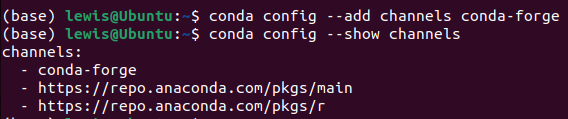
\includegraphics[width=\linewidth]{Implementation/GX/Initialisation/6.png}
    \caption{Creating a new data source (3/3)}
    \label{fig:GXDatasource3}
\end{figure}

\para Upon running the final block of code in the Jupyter notebook prompted by 
GX, the data source is finalised. Next, a suite must be created to allow for the easy creation of expectations \autocite{gx_expectation_nodate}.

\begin{figure}[H]
    \centering
    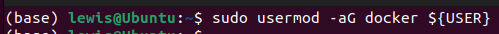
\includegraphics[width=\linewidth]{Implementation/GX/Initialisation/7.png}
    \caption{Creating a new suite (1/2)}
    \label{fig:GXSuite1}
\end{figure}

\begin{figure}[H]
    \centering
    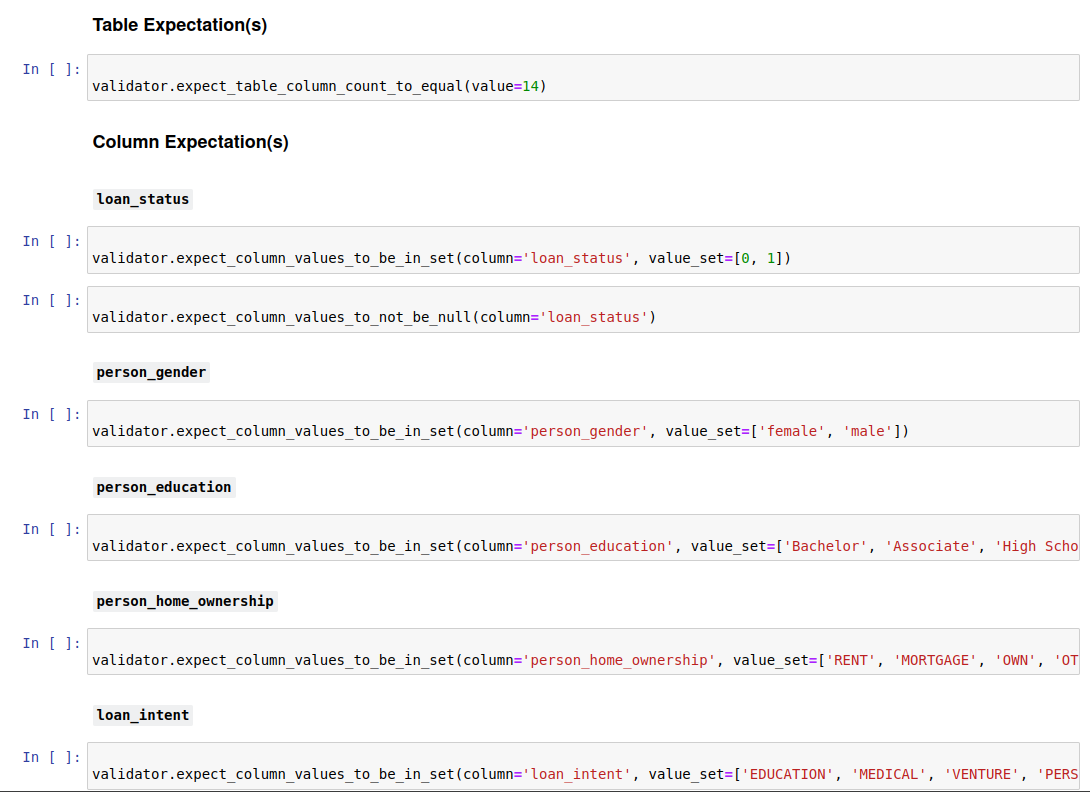
\includegraphics[width=.75\linewidth]{Implementation/GX/Initialisation/8.png}
    \caption{Creating a new suite (2/2). The full list of expectations is in Table \ref{tab:Expectations}.}
    \label{fig:GXSuite2}
\end{figure}

\begin{longtable}{ | p{0.4\textwidth} | p{0.5\textwidth} |}
    \hline
    \cellcolor{blue!25}Item & \cellcolor{blue!25}Expectation\\
    \hline
    Dataset & Must be exactly 14 columns. \\
    \hline
    loan\_status & Must not be null. \newline Must be 0 or 1. \\
    \hline 
    person\_gender & Must be 'female' or 'male'. \\
    \hline 
    person\_education & Must be 'Bachelor', 'Associate', 'High School', 'Master', or 'Doctorate'. \\
    \hline
    person\_home\_ownership & Must be 'RENT', 'MORTGAGE', 'OWN', or 'OTHER'.\\
    \hline 
    loan\_intent & Must be 'EDUCATION', 'MEDICAL', 'VENTURE', 'PERSONAL', 'DEBTCONSOLIDATION', or 'HOMEIMPROVEMENT'.\\
    \hline 
    previous\_loan\_defaults\_on\_file & Must be 'Yes' or 'No'. \\
    \hline
    credit\_score & Must be between 350 and 900. \\
    \hline
    cb\_person\_cred\_hist\_length & Must be between 0 and 30. \\
    \hline
    loan\_percent\_income & Must be between 0 and 0.8. \\
    \hline
    loan\_int\_rate & Must be between 5.0 and 30.0. \\
    \hline
    loan\_amnt & Must be between 0 and 50,000. \\
    \hline 
    person\_emp\_exp & Must be between 0 and 125. \\
    \hline 
    person\_income & Must be greater than 5000. \\
    \hline 
    person\_age & Must be greater than 0. \\
    \hline
\caption{Expectations set for the dataset and its columns.}\label{tab:Expectations}
\end{longtable}

